
\de{ĐỀ THI ÔN TẬP  HỌC KỲ II NĂM HỌC 2022-2023}{THPT Tây Thạnh}



%%=====Bài 1
\begin{bt}%[Dự Án Đề Thi HK2-K10-2022-2023]%[Nguyễn Văn Sang]%[0D8B3-1]
Viết khai triển và tìm số hạng chứa $x^3$ của khai triển nhị thức Newton $(2x-3)^5$.
\loigiai{
Khai triển nhị thức Newton của  $(2x-3)^5$, ta được
\begin{eqnarray*}
	(2x-3)^5&=&\mathrm{C}_5^0(2x)^5+\mathrm{C}_5^1(2x)^4(-3)^1+\mathrm{C}_5^2(2x)^3(-3)^2\\
	&& +\, \mathrm{C}_5^3(2x)^2(-3)^3+\mathrm{C}_5^4(2x)^5(-3)^4+\mathrm{C}_5^5(-3)^5\\
	        &=&32x^5-240x^4+720x^3-1080x^2+810x-243.
\end{eqnarray*}
Từ khai triển, ta được số hạng chứa $x^3$ là $720x^3$.
}
\end{bt}

%%=====Bài 2
\begin{bt}%[Dự Án Đề Thi HK2-K10-2022-2023]%[Nguyễn Văn Sang]%[0D8Y1-1]
Cho tập $A=\{1;2;3;4;5;6;7\}$. Hỏi có bao nhiêu số tự nhiên có $4$ chữ số khác nhau đôi một được lập từ $A$?
\loigiai{
\begin{itemize}
	\item Cách $1$: Dùng phép đếm.\\
	Gọi $\overline{abcd}$ là số tự nhiên có $4$ chữ số khác nhau đôi một được lập từ $A$.
	\begin{itemize}
		\item $a\in A$ suy ra $a$ có $7$ cách chọn.
		\item $b\in A\setminus \{a\}$ suy ra $b$ có $6$ cách chọn.
		\item $c\in A\setminus \{a,b\}$  suy ra $c$ có $5$ cách chọn.
		\item $d\in A\setminus \{a,b,c\}$ suy ra $d$ có $4$ cách chọn.
	\end{itemize}
	Theo quy tắc nhân, ta được $7\cdot6\cdot5\cdot4=840$ số.
	\item Cách $2$: Dùng chỉnh hợp.\\
	Số tự nhiên có $4$ chữ số khác nhau đôi một được lập từ $A$ là một chỉnh hợp chập $4$ của $7$ phần tử.\\
	Vậy có $\mathrm{A}_7^4=7\cdot6\cdot5\cdot4=840$ số.
\end{itemize}
}
\end{bt}

%%=====Bài 3
\begin{bt}%[Dự Án Đề Thi HK2-K10-2022-2023]%[Nguyễn Văn Sang]%[0D8B2-1]
Một tổ có $12$ học sinh. Hỏi có bao nhiêu cách chia $12$ học sinh ra làm $4$ nhóm $A$, $B$, $C$ và $D$ sao cho mỗi nhóm có số học sinh bằng nhau?
\loigiai{
Do có $12$ học sinh chia đều ra $4$ nhóm với số học sinh bằng nhau nên mỗi nhóm có $3$ học sinh.\\
Chọn $3$ học sinh vào nhóm $A$ có $\mathrm{C}_{12}^3$ cách.\\
Chọn $3$ học sinh vào nhóm $B$ có $\mathrm{C}_9^3$ cách.\\
Chọn $3$ học sinh vào nhóm $C$ có $\mathrm{C}_6^3$ cách.\\
Chọn $3$ học sinh vào nhóm $D$ có $\mathrm{C}_3^3$ cách.\\
Vậy có $\mathrm{C}_{12}^3\cdot\mathrm{C}_9^3\cdot\mathrm{C}_6^3\cdot\mathrm{C}_3^3=369600$ cách.
}
\end{bt}

%%=====Bài 4
\begin{bt}%[Dự Án Đề Thi HK2-K10-2022-2023]%[Nguyễn Văn Sang]%[0H9B3-2]
Trong mặt phẳng tọa độ $Oxy$, cho hai điểm $A(-5;2), B(1;4)$. Viết phương trình đường tròn có đường kính $AB$.
\loigiai{
\immini
{
Gọi $I$ là tâm đường tròn đường kính $AB$.\\
Suy ra $I$ là trung điểm $AB$ và $I(-2;3)$.\\
Ta có $\overrightarrow{IA}=(-3;-1)$ và bán kính  $R=IA=\sqrt{10}$.\\
Phương trình đường tròn đường kính $AB$ là 
$$ (C)\colon (x+2)^2+(y-3)^2=10.$$
}
{
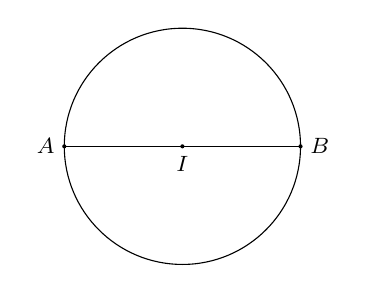
\begin{tikzpicture}[scale=.75, font=\footnotesize, line join=round, line cap=round, >=stealth]
	\draw (0,0) circle (2cm);
	\fill (-2,0) circle (1pt) node[left]{$A$};
	\fill (2,0) circle (1pt) node[right]{$B$};
	\fill (0,0) circle (1pt) node[below]{$I$}; 
	\draw (-2,0)--(2,0);
\end{tikzpicture}
}
}
\end{bt}

%%=====Bài 5
\begin{bt}%[Dự Án Đề Thi HK2-K10-2022-2023]%[Nguyễn Văn Sang]%[0H9B4-1]
Trong mặt phẳng tọa độ $Oxy$, cho Elip $(E)$ có phương trình $\dfrac{x^2}{9}+16y^2=1$. Tìm độ dài trục lớn, trục bé và các tiêu điểm của Elip.
\loigiai{
\immini
{
Chuyển Elip $(E)$ về dạng phương trình chính tắc
$$\dfrac{x^2}{9}+16y^2=1\Leftrightarrow \dfrac{x^2}{9}+\dfrac{y^2}{\tfrac{1}{16}}=1.$$
}
{
\begin{tikzpicture}[scale=1.25, font=\footnotesize, line join=round, line cap=round, >=stealth]
	\draw (0,0) ellipse (3cm and 0.35cm); % Vẽ đường elip tâm O có trục lớn 4cm và trục nhỏ 2cm
	\draw[->] (-4,0) -- (4,0) node[below] {$x$};
	\draw[->] (0,-1) -- (0,1) node[right] {$y$};
	\fill (0,0) circle (1pt) node[below left]{$O$};
	\fill (2.8,0) circle (1pt) node[below right]{$F_2$}; 
	\fill (-2.8,0) circle (1pt) node[below left]{$F_1$}; 
\end{tikzpicture}
}\noindent
Ta được $a=3$, $b=\dfrac{1}{4}$ và $c=\sqrt{a^2-b^2}=\dfrac{\sqrt{143}}{4}$.\\
Khi đó
\begin{itemize}
	\item Độ dài trục lớn là $2a=6$.
	\item Độ dài trục bé là $2b=\dfrac{1}{2}$.
	\item Các tiêu điểm là $F_1\left( -\dfrac{\sqrt{143}}{4};0\right) $ và $F_2\left( \dfrac{\sqrt{143}}{4};0\right) $.
\end{itemize}
}
\end{bt}

\begin{bt}%[0T9Y4-5]%[Dự Án Đề Thi HK2-K10-2022-2023]%[TheHung Nguyen]
Trong mặt phẳng toạ độ $Oxy$, viết phương trình chính tắc của Parabol $(P)$, biết parabol đi qua điểm $A(1 ;-4)$.
\loigiai{Phương trình chính tắc của parabol có dạng  $(P)\colon y^2=2 p x$ với $p>0$.\\
	Vì $A(1 ;-4)\in (P)$ nên $(-4)^2=2\cdot p\cdot 1\Leftrightarrow p=8$.\\
	Vậy $(P)\colon y^2=16x$.
}
\end{bt}

\begin{bt}%[0T9B3-3]%[Dự Án Đề Thi HK2-K10-2022-2023]%[TheHung Nguyen]
Trong mặt phẳng với hệ trục toạ độ $Oxy$, cho đường tròn $(C)$ có phương trình $x^2+y^2-2 x+6 y-7=0$. Viết phương trình tiếp tuyến của đường tròn $(C)$, biết tiếp tuyến vuông góc với đường thẳng $(\Delta)\colon\heva{&x=2+t\\ &y=3-4t}$.
	\loigiai{Đường tròn $(C)$ có tâm $I(1;-3)$ và bán kính $R=\sqrt{1^2+(-3)^2-(-7)}=\sqrt{17}$.\\
		Ta có $\heva{&x=2+t\\ &y=3-4t}\Rightarrow \heva{&4x=8+4t\\ &y=3-4t}\Rightarrow 4x+y-11=0$.\\
	Do đó phương trình tổng quát của $(\Delta)$ có phương trình $4x+y-11=0$.\\
	Gọi $(d)\colon x-4y+c=0$ là đường thẳng vuông góc với $(\Delta)$.\\
	Để $(d)$ là tiếp tuyến của $(C)$ thì $$\mathrm{d}(I, d)=R\Leftrightarrow \dfrac{|1-4\cdot (-3)+c|}{\sqrt{1^2+(-3)^2}}=\sqrt{17}\Leftrightarrow |13+c|=17\Leftrightarrow \hoac{& c=4 \\ & c=-30.}$$
	Vậy tiếp tuyến thỏa đề bài là $x-4y+4=0$ và $x-4y-30=0$.
	}
\end{bt}

\begin{bt}%[0T8B2-2]%[Dự Án Đề Thi HK2-K10-2022-2023]%[TheHung Nguyen]
Một tổ có $10$ học sinh, giáo viên muốn xếp $10$ học sinh đó vào $5$ bàn, mỗi bàn $2$ bạn. Trong số $10$ bạn đó có môt bạn tên Hà và một bạn tên Thảo. Hỏi có bao nhiêu cách xếp chỗ cho 10 bạn đó, biết rằng Thảo không xếp ngồi cùng bàn với Hà.
	\loigiai{
		\begin{itemize}
		\item Xếp Thảo vào $1$ trong $10$ chỗ ngồi nên có $10$ cách xếp.
		\item Vì mỗi bàn có $2$ chỗ ngồi và Hà với Thảo không ngồi cạnh nhau nên có $8$ cách xếp Hà vào $8$ chỗ ngồi.
		\item Xếp $8$ bạn còn vào $8$ chỗ ta có $8!$ cách xếp.
		\end{itemize}	
	Theo quy tắc nhân ta có $10\cdot 8\cdot8!=3225600$ cách xếp.
	}
\end{bt}

\begin{bt}%[0T9B3-6]%[Dự Án Đề Thi HK2-K10-2022-2023]%[TheHung Nguyen]
	Bạn Bảo đã trang trí thêm phụ kiện cho xe đạp nên bạn có gắn thêm một chuông 
	\immini{ở một điểm $C$ nằm chính giữa tay cầm của xe, một bóng đèn để chiếu sáng ban đêm tại một điểm $B$ trên bánh xe. Biết khoảng cách từ trục của bánh xe (tâm $I$ đường tròn) đến chuông là $50$cm. Tính bán kính của bánh xe, biết rằng đường thẳng qua hai điểm $B$ và $C$ tiếp xúc với bánh xe và chu vi tam giác $ICB$ bằng $120$cm.}{\definecolor{battleshipgrey}{rgb}{0.52, 0.52, 0.51}
		\begin{tikzpicture}[line join=round, line cap=round,scale=1.25,transform shape]
			\clip (-3.5,-2) rectangle (0,1);
			
			\tikzset{banh_xe/.pic={
					\draw[fill=battleshipgrey] (-1.75,-.78) circle (31pt);
					\draw[fill=white] (-1.75,-.78) circle (26pt);
					%------------------------------
					\draw (-1.7,-.79)--(-1.1,-1.44) (-1.8,-.86)--(-1.45,-1.65) (-1.74,-.86)--(-1.8,-1.7) (-1.8,-.86)--(-2.05,-1.65) (-1.74,-.86)--(-2.3,-1.5)(-1.85,-.86)--(-2.48,-1.33) (-1.85,-.86)--(-2.63,-1) (-1.85,-.75)--(-2.66,-.7) (-1.88,-.79)--(-2.55,-.35) (-1.86,-.75)--(-2.2,0) (-1.75,-.73)--(-2.4,-0.15) (-1.8,-.7)--(-1.75,.13)(-1.73,-.8)--(-1.05,-.2) (-1.76,-.87)--(-.9,-.47) (-1.76,-.75)--(-.83,-.82) (-1.76,-.75)--(-1.33,.03) (-1.77,-.85)--(-.93,-1.2); 
			}}
			\path
			(0,0)pic[scale=1]{banh_xe};
			\path 	(-2,.285) coordinate (B)
			(-1.78,-.77) coordinate (I)
			(-.6,.6) coordinate (C)
			;
			\draw [red](B)--(C)--(I)--cycle ;
			\draw[line width=1] (-.7,.9)--(-.5,.35);
			\draw pic[draw=red, angle radius=.1cm]{right angle=I--B--C};
			\node[red] at (I) [below right]{\tiny $I$};
			\node[red] at (C) [right]{\tiny $C$};
			\node[red] at (B) [above]{\tiny $B$};
			\draw[fill=black!70] (-1.79,-.79) circle (2.3pt);
	\end{tikzpicture}}
\loigiai{Ta có chu vi $\triangle IBC$ bằng $120$cm nên $IB+BC+CI=120\Rightarrow IB+BC=70\Rightarrow BC=70-IB$.\\
	Theo định lý Pi-ta-go trong $\triangle IBC$ vuông tại $B$ nên ta có $$IB^2+BC^2=CI^2\Rightarrow IB^2+(70-IB)^2=50^2\Rightarrow IB^2-70\cdot IB-1200=0\Rightarrow \hoac{& IB=30 \\ & IB=40.}$$
	Vậy bán kính của xe thỏa đề bài là $30$cm, $40$cm.
}
\end{bt}

\begin{bt}%[0T9B4-0]%[Dự Án Đề Thi HK2-K10-2022-2023]%[TheHung Nguyen]
Hai tháp vô tuyến $A$ và $B$ cách nhau $200$ km được đặt dọc bờ biền. Các tín hiệu được gửi đồng thời từ con tàu đến mỗi tháp và tín hiệu ở $B$ nhận sớm hơn ở $A$ là $0,0005s$ s. Giả sừ rằng các tín hiệu được truyền đi với vận tốc $300000 \mathrm{~km} / \mathrm{s}$.
\begin{enumerate}
	\item Hãy viết phương trình chính tắc của quỹ đạo hypebol $(H)$ của con tàu. 
	\item Giả sử con tàu cách trục đối xứng của $A B$ một đoạn $80$km. Hỏi con tàu cách tháp $A$ bao xa? $181{,}67$km.
\end{enumerate}
\loigiai{
	\begin{enumerate}
	\item  	Phương trình chính tắc của hybebol có hạng $(H)\colon \dfrac{x^2}{a^2}-\dfrac{y^2}{b^2}=1$ với $a>0$, $b>0$.\\	
	Gọi hai trạm phát tín hiệu vô tuyến đặt tại hai vị trí $A$, $B$ lần lượt là hai tiêu điểm của hypebol cần tìm $\Rightarrow AB=2c=200\Rightarrow c=100$.\\
Nên tọa độ hai điểm là $A(-100 ; 0)$ và $B(100 ; 0)$.\\
Khi đó ta xem vị trí tàu thủy là điểm $M$ nằm trên hypebol có $2$ tiêu điểm lần lượt là $A$ và $B$.\\
Do tín hiệu ở $B$ nhận sớm hơn tín hiệu ở $A$ nên ta có $MA-MB=300000\cdot 0{,}0005=150$.\\
mà $MA-MB=2a$ nên $2a=150\Rightarrow a=75$.\\
Mặt khác ta có $b^2=c^2-a^2=100^2-75^2=4375$.\\
Vậy phương trình chính tắc của quỹ đạo hypebol $(H)$ của con tàu là $\dfrac{x^2}{5625}-\dfrac{y^2}{4375}=1$.
\item Gọi $E(80,y)\in (H)$, khi đó ta có $\dfrac{80^2}{5625}-\dfrac{y^2}{4375}=1\Rightarrow y^2=\dfrac{5425}{9}\Rightarrow \hoac{& y=\dfrac{5\sqrt{217}}{3}~(\text{nhận}) \\ & y=-\dfrac{5\sqrt{217}}{3}~(\text{loại}).}$
\immini{
	Ta có $\overrightarrow{AE}=\left(180;\dfrac{5\sqrt{217}}{3}\right)\\
	\Rightarrow AE=\sqrt{180^2+\left(\dfrac{5\sqrt{217}}{3}\right)^2}=\dfrac{545}{3}$.\\
	Vậy khi con tàu cách trục đối xứng của $AB$ một đoạn $80$km thì nó cách tháp $A$ là $\dfrac{545}{3}$km.}{\begin{tikzpicture}[scale=1, font=\footnotesize, line join=round, line cap=round, >=stealth]
		\def\a{1.2};
		\def\b{1};
		\pgfmathsetmacro\c{sqrt((\a)^2+(\b)^2)};
		\draw[->] ($(-{\a},0)-(1.5,0)$)--($({\a},0)+(1.5,0)$) node[above]{$x$};
		\draw[->] ($(0,-{\b})-(0,1)$)--($(0,{\b})+(0,1)$) node[left]{$y$};
		\draw[name path=h1,smooth, samples=200, domain=\a:2.5] plot (\x,{((\b)/(\a))*sqrt((\x)^2-(\a)^2)});
		\draw[yscale=-1,name path=h2,smooth, samples=200, domain=\a:2.5] plot (\x,{((\b)/(\a))*sqrt((\x)^2-(\a)^2)});
		\draw[xscale=-1,name path=h2,smooth, samples=200, domain=\a:2.5] plot (\x,{((\b)/(\a))*sqrt((\x)^2-(\a)^2)});
		\draw[xscale=-1,yscale=-1,name path=h2,smooth, samples=200, domain=\a:2.5] plot (\x,{((\b)/(\a))*sqrt((\x)^2-(\a)^2)});
		\def\xm{2};
		\pgfmathsetmacro\ym{((\b)/(\a))*sqrt((\xm)^2-(\a)^2)};
		\path
		(0,0) coordinate (O)
		(-\c,0) coordinate (F_1)
		(\c,0) coordinate (F_2)
		(-\a,0) coordinate (A_1)
		(\a,0) coordinate (A_2)
		(\xm,\ym) coordinate (M)
		;
		\draw[fill=black] (O) circle(1pt) node[below left]{$O$};
		\draw[fill=black] (F_1) circle(1pt) node[below]{$A$};
		\draw[fill=black] (F_2) circle(1pt) node[below]{$B$};
		\draw[fill=black] (M) circle(1pt) node[right]{$E(x;y)$};
		\draw (F_1)--(M)--(F_2);
\end{tikzpicture}}
	\end{enumerate}
}
\end{bt}
